\documentclass[12pt]{article}

\author{Jesse E.J. op den Brouw\thanks{\texttt{J.E.J.opdenBrouw@hhs.nl}}\\[2ex]The Hague University of Applied Sciences}
\title{A Minimal RISC-V processor in VHDL}
\date{\today\\[2ex]\normalsize\url{https://github.com/jesseopdenbrouw/riscv-minimal}}

\usepackage[a4paper,inner=1.0in,outer=1.2in,top=1in,bottom=1.5in,footskip=0.4in,showframe]{geometry}
\usepackage{graphicx}
\usepackage{xcolor}
\usepackage[charter]{mathdesign}
\usepackage[scale=0.92]{nimbusmono}
\usepackage{booktabs}
\usepackage{mathtools}
\usepackage{rotating}
\usepackage{register}
\usepackage[english]{babel}
\usepackage{booktabs}

%% Making captions nicer...
\usepackage[font=footnotesize,format=plain,labelfont=bf,textfont=sl]{caption}
\usepackage[labelformat=simple,font=footnotesize,format=plain,labelfont=bf,textfont=sl]{subcaption}
\captionsetup[figure]{format=hang,justification=centering,singlelinecheck=off,skip=2ex}
\captionsetup[table]{format=hang,justification=centering,singlelinecheck=off,skip=2ex}
\captionsetup[subfigure]{format=hang,justification=centering,singlelinecheck=off,skip=2ex}
\captionsetup[subtable]{format=hang,justification=centering,singlelinecheck=off,skip=2ex}
%% Put parens around the subfig name (a) (b) etc. Needs labelformat simple
\renewcommand\thesubfigure{(\alph{subfigure})}
\renewcommand\thesubtable{(\alph{subtable})}

% Parskip et al.
\usepackage{parskip}
\makeatletter
\setlength{\parfillskip}{00\p@ \@plus 1fil}
\makeatother

\usepackage{textcomp}
\usepackage{listings}
\lstset{
    basicstyle = \ttfamily,
    numbers = left,
    numberstyle=\tiny\color{gray},
    breaklines = true,
    showspaces = false,
    prebreak = \raisebox{-0.5ex}[0ex][0ex]{\color{red}\ensuremath{\hookleftarrow}},
    postbreak = \raisebox{-0.5ex}[0ex][0ex]{\color{red}\ensuremath{\hookrightarrow}},
    upquote = true,
}

\usepackage{tikz}
\usetikzlibrary{backgrounds,shapes,arrows,automata,decorations.pathreplacing}

\usepackage{hyperref}
\hypersetup{colorlinks}

\begin{document}
\maketitle

\vfill
\begin{abstract}
\parskip=0.5\baselineskip
\noindent
The RISC-V Instruction Set Architecture (ISA) is an open source instruction set for a processor. This means that anybody can create a processor that uses this instruction set. There are already processors available such as E2-core from SiFive. More freeware cores are available on several platforms (e.g. on GitHub). This documents describes a basic 32-bit RISC-V core in VHDL. The core can execute the RV32IM unprivileged instruction set, and most of the instructions from the privileged instruction set. The processor incorporates a ROM, RAM, some simple I/O, a CSR and LIC (local interrupt controller). It is targeted for implementation on an FPGA. It is tested on an Intel Cyclone V with a DE0-CV development board from Terasic with the use of Quartus Prime Lite 21.1 and QuestaSim Intel Starter Edition 2021.2. The GNU C-compiler for RISC-V is used for software development. Many C programs were successfully tested using the GNU C compiler. C++ is currently not supported.

\noindent
This processor is not intended as a replacement for commercial available processors. It is intended as a study object for Computer Science students.

\noindent
The processor has a simple two-stage pipeline and executes each instruction in two clock cycles, but the next instruction is fetched while the current instruction is executed. Jump/branches taken require two clock cycles. ROM and RAM reads need an extra clock cycle. This processor also has a basic Control and Status Registers (CSR) set, suitable to handle traps, and a hardware multiplier/divider.

\noindent
This is work in progress. Things will certainly change in the future.
\end{abstract}
\vfill

\clearpage
\tableofcontents

\clearpage
\section{Introduction}
This document describes the buildup of a simple, one core, RISC-V processor, completely written in VHDL. The core contains one HART (Hardware Thread). The processor is able to run a compiled C-program. C++ is currently not supported. The processor can handle the RV32IM Base Integer Instruction Set as set forward in ``The RISC-V Instruction Set Manual Volume I: Unprivileged ISA''. The processor can handle traps (interrupts/exceptions). The aim is to synthesize for a minimum clock frequency of 50\,MHz. The processor utilizes ROM, RAM and some simple I/O (including TIME and TIMECMP) effectively making it a microcontroller.

The processor requires two clock cycles to complete an instruction, but the next instruction is fetched while the current instruction is executed. Jumps, calls and branches taken require two clock cycles because an new instruction has to be fetched. Also, an extra clock cycle is needed when reading ROM or RAM (data) because ROM and RAM are implemented using onboard RAM block (which are buffered with an output register). The processor has a basic Control and Status Registers set, offering CYCLE and CYCLEH (completed clock cycles), TIME and TIMEH (time since last reset, in microseconds, shadowed from memory mapped registers), INSTRET and INSTRETH (number of retired instructions), and a basic set of CSRs to handle traps. A hardware multiplication requires three clock cycles to complete. A hardware division requires 16+2 clock cycles to complete.

The processor executes at top 1 MIPS/MHz (jump and branches taken and reading ROM/RAM for data requires an extra clock cycle, multiplications/divisions take more clock cycles). 
The processor only supports Machine mode (M mode).

\section{The processor}
The RISC-V processors consist of one \textit{core} and of the following building blocks:

\begin{itemize}
\item The registers contain intermediate data for calculations.
\item The ROM contains the program instructions and constant (read-only) data.
\item The RAM contains read-write data (mutable data).
\item The I/O is an interface with the outside world.
\item The ALU is responsible for almost all computations in the processor.
\item The PC is used to point to the currently executing instruction.
\item The Address Decoder and Data Router is an interface between the memory (ROM, RAM, I/O) and the ALU and registers.
\item The Instruction Decoder decodes the currently executing instruction and provides control signals to other building blocks.
\item The Control and Status Registers contains a basic set of register for trap handling in Machine mode.
\item The Local Interrupt Controller determines which trap request is fed to the processor/CSR.
\item The multiply/divide unit adheres the M-standard.
\end{itemize}

%A block diagram of the non-pipelined processor is shown in Figure~\ref{fig:blockdiagram}.
%
%\begin{sidewaysfigure}[!p]
%\centering
%\begin{tikzpicture}[thick,font=\sffamily\footnotesize,>=latex,scale=.75,framed,background rectangle/.style={fill=none}]
%% Demux and regs
%\draw (0,0) rectangle (1,-4) node[midway,rotate=90] {rd};
%\draw (1,0) rectangle (3,-4) node[midway,align=center] {REGS\\(32x32)};
%\draw[->] (0.3,-5) node[below] {rd} -- (0.3,-4);
%\draw[->] (0.7,-5.5) node[below] {rden} -- (0.7,-4);
%\draw (3,0) rectangle (4,-2) node[midway,rotate=90] {rs2};
%\draw[->] (3.0,0.5) node[left] {rs2} -- ++(0.5,0) -- ++(0,-0.5);
%\draw (3,-2) rectangle (4,-4) node[midway,rotate=90] {rs1};
%\draw[->] (3,-4.5) node[left] {rs1} -- ++(0.5,0) -- ++(0,0.5);
%\draw (4,-3) -- (7,-3) node[midway,above] {rs1\_data};
%\draw[->] (7,-3) -- (16,-3) node[above left] {address}; 
%\draw (4,-1) -- (8,-1) node[midway,above] {rs2\_data};
%\draw[->] (8,-1) -- (16,-1) node[above left] {data}; 
%\draw[fill=black] (8,-1) circle (2pt);
%\draw[fill=black] (7,-3) circle (2pt);
%
%% ALU
%\draw (6,-5) -- ++(7,0) node[midway,yshift=-0.8cm,font=\normalsize\sffamily] {ALU} -- ++(-1,-2) -- ++(-5,0) -- cycle;
%\draw[->] (7,-3) -- (7,-5);
%\draw[->] (8,-1) -- (8,-5);
%\draw[->] (5.5,-6) node[left] {alu\_op} -- (6.5,-6);
%\draw[->] (9.5,-7.0) -- (9.5,-8.5) -- ++(-10.5,0) -- ++(0,6.5) -- ++(1,0);
%\draw[->] (11,-4.0) node[above] {pc} -- ++(0,-1);
%\draw[->] (10,-4.0) node[above] {offset} -- ++(0,-1);
%\draw[->] (9,-2.0) node[above,xshift=3mm] {immediate} -- ++(0,-3);
%
%% Address decode and data route
%\draw (16,-0) rectangle ++(2,-17) node[midway,align=center] {Address\\Decode\\\&\\Data\\Router};
%\draw[->] (16,-4) node[above left] {data} -- ++(-4,0) -- ++(0,-1);
%\draw[->] (15,-6) node[left] {size} -- ++(1,0);
%\draw[->] (15,-7) node[left] {offset} -- ++(1,0);
%\draw[->] (15,-8) node[left] {memaccess} -- ++(1,0);
%\draw[<-] (15,-9) node[left] {waitfordata} -- ++(1,0);
%\draw[->] (18,-15.5) -- ++(1,0) node[right] {wrio};
%\draw[->] (18,-16.0) -- ++(1,0) node[right] {wrram};
%\draw[->] (18,-4) -- ++(1,0) node [right] {csrom};
%\draw[->] (18,-4.5) -- ++(1,0) node [right] {csram};
%\draw[->] (18,-5) -- ++(1,0) node [right] {csio};
%
%% Instruction decoder
%\draw (9,-10.5) rectangle ++(3,-6.5) node[midway,align=center] {Instruction\\Decoder};
%\draw[->] (12,-11.0) -- ++(1,0) node[right] {alu\_op};
%\draw[->] (12,-11.5) -- ++(1,0) node[right] {rd};
%\draw[->] (12,-12.0) -- ++(1,0) node[right] {rden};
%\draw[->] (12,-12.5) -- ++(1,0) node[right] {rs1};
%\draw[->] (12,-13.0) -- ++(1,0) node[right] {rs2};
%\draw[->] (12,-13.5) -- ++(1,0) node[right] {shift};
%\draw[->] (12,-14.0) -- ++(1,0) node[right] {immediate};
%\draw[->] (12,-14.5) -- ++(1,0) node[right] {size};
%\draw[->] (12,-15.0) -- ++(1,0) node[right] {offset};
%\draw[->] (12,-15.5) -- ++(1,0) node[right] {pc\_op};
%\draw[->] (12,-16.0) -- ++(1,0) node[right] {memacces};
%%\draw[->,red] (12,-16.5) -- ++(1,0) node[right] {error};
%\draw[->] (8,-12) node[left] {instruction} -- ++(1,0);
%\draw[->] (8,-13) node[left] {waitfordata} -- ++(1,0);
%%\draw[->,red] (8,-15) node[left] {intreq} -- ++(1,0);
%
%% ROM
%\draw (22,-1) rectangle ++(2,-3) node[midway,align=center,yshift=0.4cm] {ROM\\(control)};
%\draw[<-] (24,-2.5) -- ++(1,0) node[right] {PC};
%\draw[->] (24,-3.0) -- ++(1,0) node[right] {instruction};
%\draw[->] (18,-2) -- ++(4,0) node[midway,above] {address+offset};
%\draw (24,-1.5) -- ++(0.5,0) -- ++(0,-3) -- ++(-1,0) -- ++(0,0.5);
%\node at (24.75,-3) [rotate=90] {onboard ROM};
%
%% Address lines to RAM and I/O
%\draw[->] (21,-2) -- ++(0,-5) -- ++(1,0);
%\draw[fill=black] (21,-2) circle (2pt);
%\draw[->] (21,-7) -- ++(0,-5.5) -- ++(1,0);
%\draw[fill=black] (21,-7) circle (2pt);
%% Data lines from ROM, RAM, I/O
%\draw[->] (22,-3) -- ++(-4,0);
%\draw[->] (22,-7.5) -- ++(-4,0);
%\draw[->] (22,-13.5) -- ++(-4,0);
%% Data lines to RAM and I/O
%\draw[->] (18,-8) -- ++(1.5,0) -- ++(2.5,0);
%\draw[->] (19.5,-8) -- ++(0,-5.0) -- ++(2.5,0);
%\draw[fill=black] (19.5,-8) circle (2pt);
%
%% RAM
%\draw (22,-6) rectangle ++(2,-3) node[midway,align=center] {RAM\\(control)};
%\draw[->] (23,-10) node[below] {wrram} -- ++(0,1);
%\draw (24,-6.5) -- ++(0.5,0) -- ++(0,-3) -- ++(-1,0) -- ++(0,0.5);
%\node at (25,-8) [rotate=90] {onboard RAM};
%
%% I/O
%\draw (22,-11.5) rectangle ++(2,-3) node[midway] {I/O};
%\draw[->] (23,-15.5) node[below] {wrio} -- ++(0,1);
%\draw[<->] (24,-12.5) -- ++(1,0) node[right] {I/O lines};
%\draw[->] (24,-13) -- ++(1,0) node[right] {TxD};
%\draw[<-] (24,-13.5) -- ++(1,0) node[right] {RxD};
%%\draw[->] (24,-13.5) -- ++(1,0) node[right] {interrupts};
%
%% PC
%\draw (3,-12) rectangle ++(2,-4) node[midway] {PC};
%\draw (2,-12) rectangle ++(1,-4) node[midway, rotate=90] {mux};
%\draw[->] (5,-14) -- ++(1,0) -- ++(0,-3) -- ++ (-6,0) -- ++(0,4.333) -- ++(1,0);
%\draw[->] (6,-14) -- ++(1,0) node[right] {pc};
%\draw[fill=black] (6,-14) circle (2pt);
%\draw[->] (0,-13.5) -- ++(1,0);
%\draw[fill=black] (0,-13.5) circle (2pt);
%
%\draw (1,-12) rectangle ++(1,-1) node[midway] {+};
%\draw (1,-13) rectangle ++(1,-1) node[midway] {+4};
%\draw (1,-14) rectangle ++(1,-1) node[midway] {+};
%\draw (1,-15) rectangle ++(1,-1) node[midway] {+};
%\draw[->] (2.5,-11) node[above] {pc\_op}-- ++(0,-1);
%
%\draw[->] (1.5,-8.5) -- ++ (0,-3.5) node[xshift=-3mm,midway,rotate=90] {result(0)};
%\draw[fill=black] (1.5,-8.5) circle (2pt);
%
%\draw[->] (0,-14.6667) -- ++(1,0);
%\draw[fill=black] (0,-14.6667) circle (2pt);
%
%\draw[->] (-0.5,-11.333) node[above] {offset} -- ++(0,-1) -- ++(1.5,0);
%\draw[->] (-0.5,-12.333) -- ++(0,-2) -- ++(1.5,0);
%\draw[fill=black] (-0.5,-12.333) circle (2pt);
%\draw[->] (-0.5,-14.333) -- ++(0,-1) -- ++(1.5,0);
%\draw[fill=black] (-0.5,-14.333) circle (2pt);
%
%\draw[->] (-0.5,-17.6667) node[below] {rs1\_data} -- ++(0,2) -- ++(1.5,0);
%\end{tikzpicture}
%\caption{The complete, non-pipelined RISC-V MCU.}
%\label{fig:blockdiagram}
%\end{sidewaysfigure}



\subsection{Registers}
The register file consists of thirty-two 32-bit registers denoted by \texttt{x0} to \texttt{x31}. Internally, the registers use Big Endian format. Register \texttt{x0} (alias \texttt{zero}) is hardwired to all zeros. Writing this register has no effect. Reading this register returns all zero bits. Normally, the \texttt{x}-names are not used but may be handy when simulating the designs. Table~\ref{tab:registers} shows the names of the registers as they should be used.

A register can be written to, and two register can be selected for data and base address.

\begin{table}[!ht]
\centering
\caption{RISC-V registers and their purpose.}
\label{tab:registers}
\begin{tabular}{lllc}
Register & Name & Purpose & Saver \\
\midrule
\texttt{x0}      & \texttt{zero}   & Hard-wired zero                   & $-$ \\
\texttt{x1}      & \texttt{ra}     & Return address                    & Caller \\
\texttt{x2}      & \texttt{sp}     & Stack pointer                     & Callee \\
\texttt{x3}      & \texttt{gp}     & Global pointer                    & $-$ \\
\texttt{x4}      & \texttt{tp}     & Thread pointer                    & $-$ \\
\texttt{x5}      & \texttt{t0}     & Temporary/alternate link register & Caller \\
\texttt{x6-x7}   & \texttt{t1-t2}  & Temporaries                       & Caller \\
\texttt{x8}      & \texttt{s0/fp}  & Saved register/frame pointer      & Callee \\
\texttt{x9}      & \texttt{s1}     & Saved register                    & Callee \\
\texttt{x10-x11} & \texttt{a0-a1}  & Function arguments/return values  & Caller \\
\texttt{x12-x17} & \texttt{a2-a7}  & Function arguments                & Caller \\
\texttt{x18-x27} & \texttt{s2-s11} & Saved registers                   & Callee \\
\texttt{x28-x31} & \texttt{t3-t6}  & Temporaries                       & Caller
\end{tabular}
\end{table}

\subsection{ROM}
\label{sec:rom}
The ROM consists of bytes and is only word addressable for instructions. The ROM is byte, half word and word addressable when reading constant data. Half word and word entries are in Litte Endian format. When reading data from the ROM, half word accesses must be on 2-byte boundaries and word accesses must be on 4-byte boundaries. This simplifies the decoding circuitry. The ROM returns undefined data if an access is not aligned. The processor instantiates the ROM in onboard RAM. Rearranging half word and word data accesses in Big Endian format is handled by the ROM decoding unit.

Note: the Cyclone V has 3,153,920 bits of onboard RAM available. Because of the 32-bit entries a maximum of 2,097,152 (65536 x 32) bits can be instantiated. This is equivalent to 262,144 bytes.

\subsection{RAM}
\label{sec:ram}
The RAM consists of bytes and is byte, half word and word addressable. Half word and word entries are in Little Endian format. The RAM itself is made up of word (i.e. 32-bit) entries and is instantiated with onboard RAM blocks. Due to this fact, half word accesses are only permitted on 2-byte boundaries and word accesses are only permitted on 4-byte boundaries. The RAM returns undefined data if an access is not aligned. Writes will not take place if an access is unaligned. This simplifies the decoding circuitry. For the Cyclone V a maximum of 65536 words of RAM can be instantiated. Rearranging half word and word data accesses in Big Endian format is handled by the RAM decoding unit. The RAM cannot be used for program data.

Note: the Cyclone V has 3,153,920 bits of onboard RAM available. Because of the 32-bit entries a maximum of 2,097,152 (65536 x 32) bits can be instantiated. This is equivalent to 262,144 bytes.

Reading the RAM (byte, half word, word) requires an extra clock cycles because the RAM output is buffered by a register. This is automatically handled by the processor.

\subsection{I/O}
\label{sec/io}
Currently, the I/O consists of one 32-bit data input and one 32-bit data output, a simple USART (well, really an UART), a simple timer and the TIME and TIMEH memory mapped time registers. Note that the I/O can only be accessed as words and the addresses must be on 4-byte boundaries. If not on a 4-byte boundaries and not word size reads/writes, reads return undefined data whereas writes will not write data. Reading and writing I/O requires one clock cycle. Note that not all I/O addresses are used.

The USART can transmit and receive data at 7, 8 or 9 bits, no/even/odd parity and 1 or 2 stop bits. Tested speeds are 9600 bps, 115200 bps and 230400 bps. Several status flags are implemented to guide transmission. Note: more identical USARTs will be added. Receive and transmitted character (local) interrupts are provided.

The timer has a 32-bit time register and increments on every clock cycle. It does not have a prescaler. It counts up to a compare match register, after which is will be loaded with 0 again. A compare match (local) interrupt is provided.

The I/O incorporates memory mapped TIMEH:TIME and TIMECMPH:TIMECMP registers. Whenever TIMEH:TIME (as viewed as a 64-bit register)is greater than or equal to TIMECMPH:TIMECMP (as viewed as a 64-bit register) an interrupt is asserted. The interrupt is negated if TIMEH:TIME is less than TIMECMPH:TIMECMP.

\subsection{ALU}
\label{sec:alu}
The Arithmetic and Logic Unit (ALU) handles all computations on data. It can add, subtract, do logic operations such as AND, OR en XOR, can shift data left or right, and sign extend byte and half word data. Some operations require two registers, some only use one register. Furthermore the ALU is also used to determine if a conditional branch should be taken. Note that the RISC-V programmer's model does not incorporate status flags as some other architectures do. This requires some extra instructions when adding or subtracting double word (64-bit) data. This is handled by the C compiler. The ALU is also used to compute the return address from unconditional function calls (JAL and JALR instructions). The data is in Big Endian format. The ALU is the only building block that can write registers. The ALU does not handle multiplications and divisions.

Note that the computation of jump target addresses is handled by the Program Counter (PC)

\subsection{PC}
\label{sec:pc}
The Program Counter contains the address of the currently fetched instruction. The address is always on a 4-byte boundary although function calls and conditional jump (JAL, JALR en B$xx$ instructions) can be on non 4-byte boundaries (the C compiler will always create 4-bytes boundaries). The PC (or rather the VHDL description of the PC) handles the address calculations of jumps and branches taken.

\subsection{Instruction Decoder}
\label{sec:instructiondecoder}
The instruction decoder decodes the instruction supplied by the ROM as pointed by the PC. An instruction is 4 bytes wide and in Little Endian order. The instruction decoder provides all control signals for the ALU, RAM, ROM, I/O, the PC, the Address Decoder, the CSR, the register file and the md unit. Some signals are directly wired to the ROM, RAM and I/O.

The processor uses a five-state FSM, see figure~\ref{fsmpipe}. The PC points to +4 of the currently executing instruction, in a sequential instruction stream. If a jump or branch taken occurs, the FSM inserts a penalty because the PC has to be loaded with the correct value and a new instruction must be fetched (Figure~\ref{fsmpipeseqstartup}). Reading RAM and ROM requires an extra state (Figure~\ref{fsmpipeseqwait}). When a multiply, divide or remainder instruction is encountered, the FSM enters the \texttt{md} state and waits for the md-unit to complete (32+2 or 16+2 clock cycles). Note that penalty, wait and start cannot occur at the same time.

\begin{figure}[!ht]
\centering
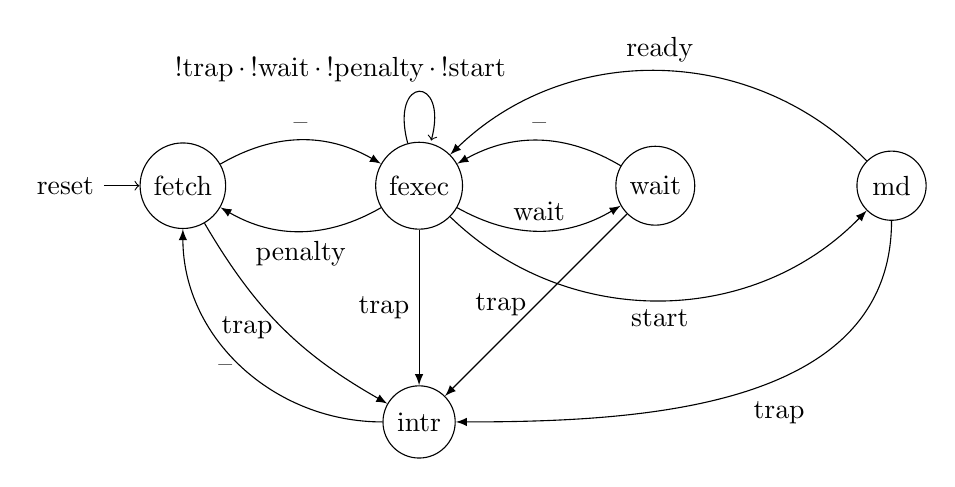
\begin{tikzpicture}[node distance=3cm]
\node[state,initial,initial text=reset] (fetch) {fetch};
\node[state,right of=fetch] (fexec) {fexec};
\node[state,right of=fexec] (wait) {wait};
\node[state,right of=wait] (md) {md};
\node[state,below of=fexec] (intr) {intr};
\path[-latex] (fetch) edge [bend left] node[above] {--} (fexec)
          (fexec) edge [bend left] node[below] {penalty} (fetch)
          (fexec) edge [bend right] node[above] {wait} (wait)
          (fexec) edge [bend right=45] node[below] {start} (md)
          (md) edge [bend right=45] node[above] {ready} (fexec)
          (wait)  edge [bend right] node[above] {--} (fexec)
          (fexec) edge [loop above] node[above,xshift=-1cm] {!trap$\,\cdot\,$!wait$\,\cdot\,$!penalty$\,\cdot\,$!start} (fexec)
          (fetch) edge [bend right=15] node[left] {trap} (intr)
          (fexec) edge node[left] {trap} (intr)
          (wait) edge node[left] {trap} (intr)
          (md) edge [out=270, in=0] node[below right] {trap} (intr)
          (intr) edge [out=180, in=270] node[left] {--} (fetch)
;
\end{tikzpicture}
\caption{FSM of the instruction decoder of the processor.}
\label{fsmpipe}
\end{figure}

\begin{figure}[!ht]
\centering
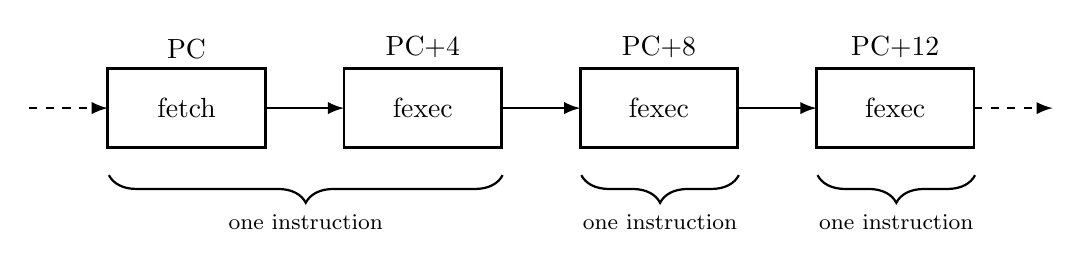
\begin{tikzpicture}[node distance=2cm, line width=1pt]
\draw[-latex,dashed] (-1,-0.5) -- ++(1,0);

\draw (0,0) rectangle node [] {fetch} ++(2,-1);
\node at (1,0) [above] {PC};
\draw[-latex] (2,-0.5) -- ++(1,0);

\draw (3,0) rectangle node [] {fexec} ++(2,-1);
\node at (4,0) [above] {PC+4};
\draw[-latex] (5,-0.5) -- ++(1,0);

\draw (6,0) rectangle node [] {fexec} ++(2,-1);
\node at (7,0) [above] {PC+8};
\draw[-latex] (8,-0.5) -- ++(1,0);

\draw (9,0) rectangle node [] {fexec} ++(2,-1);
\node at (10,0) [above] {PC+12};
\draw[-latex,dashed] (11,-0.5) -- ++(1,0);

\draw [thick,decorate,decoration={brace,amplitude=10pt,mirror},xshift=0.4pt,yshift=-10pt](0,-1) -- (5,-1) node[black,midway,yshift=-0.6cm] {\footnotesize one instruction};
\draw [thick,decorate,decoration={brace,amplitude=10pt,mirror},xshift=0.4pt,yshift=-10pt](6,-1) -- (8,-1) node[black,midway,yshift=-0.6cm] {\footnotesize one instruction};
\draw [thick,decorate,decoration={brace,amplitude=10pt,mirror},xshift=0.4pt,yshift=-10pt](9,-1) -- (11,-1) node[black,midway,yshift=-0.6cm] {\footnotesize one instruction};
\end{tikzpicture}
\caption{State sequence for start up/penalty with instruction execution (no wait state).}
\label{fsmpipeseqstartup}
\end{figure}

\begin{figure}[!ht]
\centering
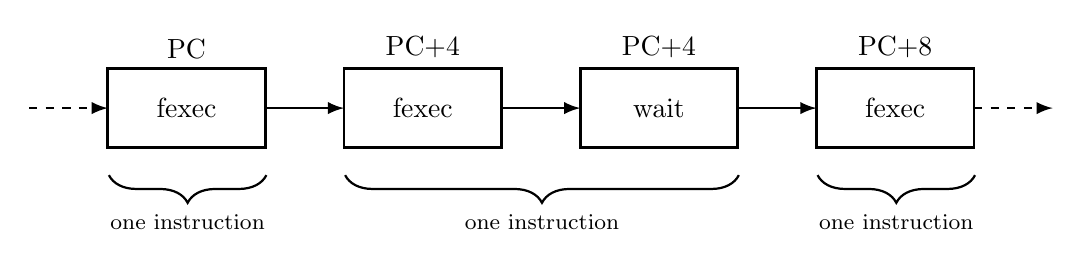
\begin{tikzpicture}[node distance=2cm, line width=1pt]
\draw[-latex,dashed] (-1,-0.5) -- ++(1,0);

\draw (0,0) rectangle node [] {fexec} ++(2,-1);
\node at (1,0) [above] {PC};
\draw[-latex] (2,-0.5) -- ++(1,0);

\draw (3,0) rectangle node [] {fexec} ++(2,-1);
\node at (4,0) [above] {PC+4};
\draw[-latex] (5,-0.5) -- ++(1,0);

\draw (6,0) rectangle node [] {wait} ++(2,-1);
\node at (7,0) [above] {PC+4};
\draw[-latex] (8,-0.5) -- ++(1,0);

\draw (9,0) rectangle node [] {fexec} ++(2,-1);
\node at (10,0) [above] {PC+8};
\draw[-latex,dashed] (11,-0.5) -- ++(1,0);

\draw [thick,decorate,decoration={brace,amplitude=10pt,mirror},xshift=0.4pt,yshift=-10pt](0,-1) -- (2,-1) node[black,midway,yshift=-0.6cm] {\footnotesize one instruction};
\draw [thick,decorate,decoration={brace,amplitude=10pt,mirror},xshift=0.4pt,yshift=-10pt](3,-1) -- (8,-1) node[black,midway,yshift=-0.6cm] {\footnotesize one instruction};
\draw [thick,decorate,decoration={brace,amplitude=10pt,mirror},xshift=0.4pt,yshift=-10pt](9,-1) -- (11,-1) node[black,midway,yshift=-0.6cm] {\footnotesize one instruction};
\end{tikzpicture}
\caption{State sequence for instruction execution (wait state).}
\label{fsmpipeseqwait}
\end{figure}

\subsubsection{Trap handling in the instruction decoder}
When an interrupt occurs, the FSM enters the \texttt{intr} state for fetching the trap vector. An interrupt can occur any time and is called asynchronous. When an interrupt occurs in the \texttt{fetch} state, the current instruction is discarded. When an interrupt occurs in the \texttt{fexec} state, the current instruction is either retired or discarded (load, mul, div, rem). In the latter case the instruction must be restarted. When occurring in the \texttt{wait} state, the instruction (load) is retired. When occurring in the \texttt{md} state \emph{and} the md unit is ready, the instruction (mul, div, rem) is retired. When occurring in the \texttt{md} state and the md unit is \emph{not} ready the instruction is discarded and must be restarted. After loading the trap vector, the FSM enters the \texttt{fetch} state.

Exceptions are synchronous to executing instructions. When occurring in the \texttt{fetch} state, the instruction is discarded and the FSM enters the \texttt{intr} state. When occurring in the \texttt{fexec} state, the instruction is either retired or discarded (load, mul, div, rem). In this case the instruction must be restarted. Note that exceptions cannot occur in the \texttt{wait} (load already started) and \texttt{md} states (not executing instructions).

When a trap request is asserted, the trap vector is loaded in the next clock cycle. Then, in the second clock cycle, the instruction is fetched and in the third clock cycle the instruction is executed. On return from a trap handler, the original contents of the PC is restored and the FSM enters the \texttt{fetch} state.


\subsection{Address Decoder and Data Router}
\label{sec:addressdecoderanddatarouter}
The Address Decoder and Data Router routes reads and writes to the ROM (only reads), RAM and the I/O. The processor uses a 32-bit linear address space for ROM, RAM and I/O. In the default setting, ROM starts at address 0x00000000 and the length is 64 kB. Unused ROM addresses return 0x0000000. The RAM starts at address 0x20000000 and length is 32 kB. The I/O starts at address 0xF0000000 and the length is 16 kB by default.

When data is read, the data is collected from the accessed memory and put on an internal bus to the ALU. The ALU can perform sign extension (byte and half word accesses) if needed. Please note that reading data from the RAM and ROM requires an extra clock cycle. Reading data from I/O requires no extra clock cycle.

Note that instructions can only be fetched from ROM.

\subsection{Control and Status registers}
The RISC-V specification describes a set of 4096 control and status register in a separate address space. Basic event counters are implemented:

\begin{itemize}
\item \texttt{cycle} and \texttt{cycleh} -- these 32-bit registers form a 64-bit value that contains the counted clock cycles since the last reset.
\item \texttt{time} and \texttt{timeh} -- these registers shadow the contents of the TIME and TIMEH registers from the I/O.
\item \texttt{instret} and \texttt{instreh} -- these 32-bit registers form a 64-bit value that contains the counted retired instructions since the last reset.
\end{itemize}

Note that these registers are read-only. Writes are ignored. 

For trap handling, the following registers are implemented:

\begin{itemize}
\item \texttt{mvendorid} -- this register is hardwired to all zero bits.
\item \texttt{marchid} -- this register is hardwired to all zero bits.
\item \texttt{mimpid} -- this register is hardwired to all zero bits.
\item \texttt{mhartid} -- this register is hardwired to all zero bits.
\item \texttt{mconfigptr} -- this register is hardwired to all zero bits.
\end{itemize}

\begin{itemize}
\item \texttt{mstatus} -- the only implemented bits are \texttt{MIE}, \texttt{MPIE} and \texttt{MPP}, all other bits are hardwired zero.
\item \texttt{misa} -- hardwired to value 0x40001100, indicating 32-bit processing, RV32I base ISA and Integer Multiply/Divide extension.
\item \texttt{mie} -- for the lower 16 bits, only \texttt{MTIE} is implemented, all other bits are hardwired zero.
\item \texttt{mtvec} -- contains the trap handler (vector) address, can be used in direct and vectored mode.
\item \texttt{mstatush} -- this register is hardwired to all zero bits.
\item \texttt{mscratch} -- currently not used, but can be used by software trap handlers.
\item \texttt{mepc} -- contains the PC at point of trap of the \emph{currently} executing instruction.
\item \texttt{mcause} -- contains the cause of the trap as set forward in ``The RISC-V Instruction Set Manual, Volume II: Privileged Architecture''. For local interrupts, additional codes are used.
\item \texttt{mtval} -- contains the address on the address bus when a trap occurs, not always relevant.
\item \texttt{mip} -- contains the pending interrupts. For the lower 16 bits, only \texttt{MTIP} is implement. The upper 16 bits are used for local interrupts. This register is read-only.
\item \texttt{mconfigptr} -- this register is hardwired to all zero bits.
\end{itemize}

The \texttt{mcounteren} and \texttt{mcountinhibit} registers are not implemented, because U-mode is not implemented. The \texttt{menvcfg} and \texttt{menvcfgh} are not implemented, because only M-mode is implemented.

The trap handler (vector) address must be loaded by software at boot time. Both direct and vectored mode are supported. In direct mode all traps redirect to a trap handler that has to handle both interrupts and exceptions. The most significant bit of \texttt{mcause} is 1 when a trap occurred from an interrupt. In vectored mode, the addresses of \emph{interrupt handlers} are loaded from a jump table. Exceptions are redirected to a single handler. Note that the address of the trap handler must be on a 4-byte boundary, and bit 0 has to be set to 1 for vectored mode.

Other CSRs are not implemented. Good synthesizers will remove not-used CSRs.

\subsection{Local Interrupt Control unit}
The Local Interrupt Controller is responsible for selecting which trap request must be serviced by the core. Interrupts have higher priority than exceptions. The state of the serviced trap is visible in the CSR.

The LIC can handle 16 local interrupts (numbered 16 to 31) and the Machine mode external timer interrupt (numbered 7). Other standard RISC-V interrupts (numbered 0 to 6 and 8 to 15) are not available. The external timer interrupt has the highest priority, followed (currently) by the USART and TIMER1 interrupts.

Exceptions are handled as set forward in Table 3.7 of ``The RISC-V Instruction Set Manual, Volume II: Privileged Architecture'': instruction access fault, instruction address misaligned, ECALL (M mode only), EBREAK, load/store address misaligned, load/store access fault. Note that ECALL and EBREAK are user instructions and can be interrupted by an interrupt (i.e. when the ECALL or EBREAK is executed).

\subsection{Multiply/Divide Unit}
The processor is equipped with a hardware multiply/divide unit. All multiply/divide instructions are supported (\texttt{MUL}, \texttt{MULH}, \texttt{MULHSU}, \texttt{MULHU}, \texttt{DIV}, \texttt{DIVU}, \texttt{REM}, \texttt{REMU}) and the result is fed to the ALU. A multiplication takes three clock cycles (one clock-in, one multiply, one clock-out). For division, two versions are available. By default, the divider needs 18 clocks (one clock-in, 16 divide, one clock-out) for a division using a poor man's radix-4 division unit. As an alternative, a simple radix-2 division unit can be selected taking 34 clock cycles (one clock-in, 32 divide, one clock-out) to do the division.  Thus, the radix-4 divider unit is faster, but needs more cells. The radix-2 divider unit is slower, but needs less cells. You have to enable the M-standard support in the compiler. The multiplier uses special DSP units in the Cyclone V. Most regular FPGAs have onboard multipliers.


\subsection{Stack pointer}
The stack pointer is fully implemented although the ISA does not provide pushes and pops. The stack pointer is used to allocate local variables and is updated with each allocation and deallocation. As usual, the stack grows downwards (to lower addresses) on allocations and upwards (to higher addresses) on deallocations. Therefore the stack pointer is set to the highest RAM address + 1 on boot (which is 0x20008000 by default). The ISA postulates that the stack is aligned on 16-byte boundaries for the I standard.

\subsection{Implemented instructions}
For the processor, all RV32IM Unprivileged instructions are implemented with the exception of the FENCE instruction. This instruction act as a no-operation (NOP). ECALL and EBREAK are supported and execute an exception. MRET is used to return from an exception or an interrupt. WFI is not supported and act as a no-operation (NOP).

\section{The FPGA}
For this project, we use the Cyclone V FPGA from Intel (formerly Altera). See \url{https://www.intel.com/content/www/us/en/products/details/fpga/cyclone/v.html}.
The used Cyclone V is the 5CEFA4F23C7 which has 18480 ALMs available. It has 3080 kb of onboard RAM bits available which are used for RAM and ROM. Depending on the program and used resources, the compiled RISC-V processor uses about 2700 ALMs (about 15\,\%) and 786,432 bits of internal memory (25\,\%). The clock frequency is 50\,MHz which is sufficient for all program examples. This FPGA is mounted on a Terasic DE0-CV board. The board has 10 switches, 4 push buttons, 1 reset push button, 10 leds, and 6 seven-segment displays. It also has two 2x20-pin headers to connect off-board devices. See \url{http://www.terasic.com.tw/cgi-bin/page/archive.pl?Language=English&No=921}. For downloading the program file, the onboard USB-Blaster is used.

It is possible to add the Quartus' Signal Tap (embedded) Logic Analyzer. Follow the instructions on \url{https://people.ece.cornell.edu/land/courses/ece5760/Quartus/Signal_tap.html}. Note that the Signal Tap uses onboard memory.

\section{Simulation}
The designs can be simulated fully, using QuestaSim Intel Starter or ModelSim Intel Starter. You need a (free) license for QuestaSim. During simulation, all essential signals can be viewed, as is the RAM. The RAM is viewed as 32-bit entries, so we need to do some manual calculations to correctly find byte, half word and word accesses. Simulation can be started from Quartus.

\section{Cloning the RISC-V project}
\label{sec:cloning}
Now we have to clone the RISC-V project. It incorporates the full Quartus Prime Lite project with the processor written in VHDL. It also incorporates some simple C program examples and a taylor-made program to convert a RISC-V executable to a VHDL table suitable for the ROM. Create a working directory (and change to that directory) and issue the command:

\begin{lstlisting}[language=]
git clone https:/github.com/jesseopdenbrouw/riscv-minimal
\end{lstlisting}

In the created directory, you will see the following directories:

\texttt{CODE} -- Sample software programs, linker script and startup files\\
\texttt{DOCS} -- Documentation\\
\texttt{HARDWARE} -- the VHDL descriptions \\
\texttt{OLD} -- yes, really old files for backup\\
\texttt{RETIRED} -- Descriptions that are not used anymore

Change directory to \texttt{CODE}. Make sure the RISC-V C compiler is available (see Section~\ref{sec:ccompiler}) and is in your path environment variable. Now enter the command \texttt{make}. It will compile all programs and the taylor-made conversion program. To clean up the programs, issue the command \texttt{make clean}.

If you want, you can compile the processor with the standard program incorporated, which is by default, flashing the onboard leds. Start your Quartus Prime Lite software and open the project in the \texttt{HARDWARE} directory. Now start a build by clicking on the play-symbol. It should compile a standard setting (this takes a long time). When finished, you can download the FPGA contents to the DE0-CV board.

To test one of the programs, change directory to one of the directories in \texttt{CODE} and copy the file with \texttt{.vhd} extension to the directory containing the VHDL description under the name \texttt{processor\_common\_rom.vhd}.
Now start Quartus and start the compilation. After a successful compilation, you can program the Cyclone V on a DE0-CV board.

\section{Setting up the GNU C compiler for \textit{this} RISC-V}
\label{sec:ccompiler}
The processor can run C programs that are compiled using the GNU C compiler for RISC-V. Besides that, a separate linker script and startup file are needed to setup the compiled code. It is possible to set up the C library for multiple RISC-V architecture versions and select a version during compilation. Building the C compiler (from Linux) is straightforward:

\begin{enumerate}
\item You need a current GNU C compiler installed or your Linux box. You also need all essential building tools:
\begin{lstlisting}[language=]
apt install autoconf automake autotools-dev curl python3 libmpc-dev libmpfr-dev libgmp-dev gawk build-essential bison flex texinfo gperf libtool patchutils bc zlib1g-dev libexpat-dev
\end{lstlisting}
\item You need the texinfo package. On Ubuntu et al.\@ issue
\begin{lstlisting}[language=]
apt install texinfo
\end{lstlisting}
\item In your home directory, enter the command
\begin{lstlisting}[language=]
git clone --recursive https://github.com/riscv/riscv-gnu-toolchain
\end{lstlisting}
\item Wait for the cloning to end (takes a long time, about 30 minutes on a Zbook G5 2020 with a 10 MB/s internet connection)
\item Change to the directory with
\begin{lstlisting}[language=]
cd riscv-gnu-toolchain
\end{lstlisting}
\item Make the \texttt{build} directory with:
\begin{lstlisting}[language=]
mkdir build; cd build
\end{lstlisting}
\item Check the current configuration with
\begin{lstlisting}[language=]
../configure --help | grep abi
\end{lstlisting}
      It should say:
\begin{lstlisting}[language=]
--with-abi=lp64d    Sets the base RISC-V ABI, defaults to lp64d
\end{lstlisting}
The toolchain is currently configured for 64-bit RISC-V. That is not what we want.
\item Enter:
\begin{lstlisting}[language=]
../configure ../configure --prefix=/opt/riscv32 --with-arch=rv32i --with-abi=ilp32 --with-multilib-generator=``rv32i-ilp32--;rv32e-ilp32e--''
\end{lstlisting}
This will set the architecture to RV32I and RV32E (reduced registers), and the ABI to ilp32 and ilp32e (reduced registers). This means that integers, long integers and pointers use 32-bit entities. The destination directory is \lstinline|/opt/riscv32|.

If you wish to enable the multiply/divide instructions, issue:
\begin{lstlisting}[language=]
../configure ../configure --prefix=/opt/riscv32 --with-arch=rv32im --with-abi=ilp32
\end{lstlisting}

\item Now enter the make command as root: \lstinline|make|\\
MAKE SURE TO ENTER THIS COMMAND AS root, because the toolchain is put in \lstinline|/opt/riscv32|. This takes a long time (about 45 minutes on a Zbook G5). At some points the compilation seems to hang, but it is just compiling complicated C-files. By the way, you will see a lot of warnings.
\item Now that the toolchain is setup, we have to put the path into the \lstinline|$PATH| environment variable so enter
\begin{lstlisting}[language=]
export PATH=/opt/riscv32/bin:$PATH
\end{lstlisting}
\item Check if the compiler is available:
\begin{lstlisting}[language=]
riscv32-unknown-elf-gcc -v
\end{lstlisting}
It should say something like:
\begin{lstlisting}[language=]
Using built-in specs.
COLLECT_GCC=riscv32-unknown-elf-gcc
COLLECT_LTO_WRAPPER=/opt/riscv32/libexec/gcc/riscv32-unknown-elf/11.1.0/lto-wrapper
Target: riscv32-unknown-elf
Configured with: /mnt/d/PROJECTS/riscv-gnu-toolchain/build/../riscv-gcc/configure --target=riscv32-unknown-elf --prefix=/opt/riscv32 --disable-shared --disable-threads --enable-languages=c,c++ --with-system-zlib --enable-tls --with-newlib --with-sysroot=/opt/riscv32/riscv32-unknown-elf --with-native-system-header-dir=/include --disable-libmudflap --disable-libssp --disable-libquadmath --disable-libgomp --disable-nls --disable-tm-clone-registry --src=../../riscv-gcc --enable-multilib --with-multilib-generator='rv32i-ilp32--;rv32e-ilp32e--' --with-abi=ilp32 --with-arch=rv32i --with-tune=rocket 'CFLAGS_FOR_TARGET=-Os   -mcmodel=medlow' 'CXXFLAGS_FOR_TARGET=-Os   -mcmodel=medlow'
Thread model: single
Supported LTO compression algorithms: zlib
gcc version 11.1.0 (GCC) 
\end{lstlisting}
\end{enumerate}

\subsection{Register subset}
It is possible to compile the toolchain to only use register \texttt{x0} to \texttt{x15}. This is called the RISC-V E extension. As a positive side effect, the register file can be cut down from 32 registers to 16 registers, saving 512 memory element. This will lower the ALM (cell) count and possible speed up the device. A negative side effect is that the pressure on register allocation is higher, possibly increasing instruction count when saving registers on the stack.

Using the above recipe, the toolchain is set up for both RV32I and RV32E. You need the specify the architecture and ABI during compile time of the RISC-V programs.

Now compile a C program with:

\begin{lstlisting}[language=]
riscv32-unknown-elf-gcc -O2 -g -o flash flash.c -Wall -T ../ldfiles/riscv.ld -march=rv32e -mabi=ilp32e -nostartfiles --specs=nano.specs ../crt/startup.c
\end{lstlisting}

Make sure to use \texttt{-march=rv32e} and \texttt{-mabi=ilp32e}.


\section{Compiling a C program by hand}
We tested a large amount of programs with and without trap handling. We tested all I/O. We did test the use of the C library (\texttt{malloc} et al, floats and double calculation, some trigonometry functions from the mathematical library), but more tests are needed.

Compiling a program requires the following steps:

\begin{itemize}
\item In the program directory \lstinline|CODE|, create a new directory and change to that directory.
\item Create a C program file, we assume \lstinline|flash.c|.
\item Now issue the command:
\begin{lstlisting}[language=]
riscv32-unknown-elf-gcc -O2 -g -o flash flash.c -Wall -T ../ldfiles/riscv.ld -march=rv32i -nostartfiles --specs=nano.specs ../crt/startup.c
\end{lstlisting}
We supply our own linker file (\lstinline|-T ../ldfiles/riscv.ld|) and we supply our own startup file (\lstinline|../crt/startup.c|). Make sure to use \lstinline|-nostartupfiles| otherwise the default startup file will be linked and errors will report. There a three startup files:
\begin{itemize}
\item \texttt{empty.S} -- Empty startup file only providing the entry symbol. Can be used with assembler programs.
\item \texttt{minmal.S} -- Provides the entry symbol, loads the global pointer and stack pointer. Can be used with assembler programs.
\item \texttt{startup.S} -- Provides the entry symbol, loads the global pointer and stack pointer and calls \texttt{main}. On return of \texttt{main}, it waits in an endless loop. Can be used with minimalistic C programs.
\item \texttt{startup.c} -- Full support for C programs. Can be used with \texttt{malloc} et al.
\end{itemize}
\item Next issue the command:
\begin{lstlisting}[language=]
riscv32-unknown-elf-objcopy -O srec flash flash.srec
\end{lstlisting}
This will create an S-record file in Motorola hex-format.
\item Next issue the command:
\begin{lstlisting}[language=]
../bin/srec2vhdl -wf flash.srec flash.vhd
\end{lstlisting}
This will create a VHDL file with the ROM encoded as 32-bit Little Endian quantities. Note: the taylor-made \texttt{srec2vhdl} has to be compiled before. See Section~\ref{sec:cloning}.
\item Next issue the command:
\begin{lstlisting}[language=]
cp flash.vhd ../../HARDWARE/riscv-pipe-csr-md-lic/processor_common_rom.vhd
\end{lstlisting}
This will copy the VHDL file to the RISC-V processor ROM file.
\item Now start the compilation of the VHDL code in Quartus Prime Lite and program the compiled file. This file has the extension \lstinline|.sof|. See Figures~\ref{quartus1} to~\ref{programmer}.

\begin{figure}[!ht]
\centering
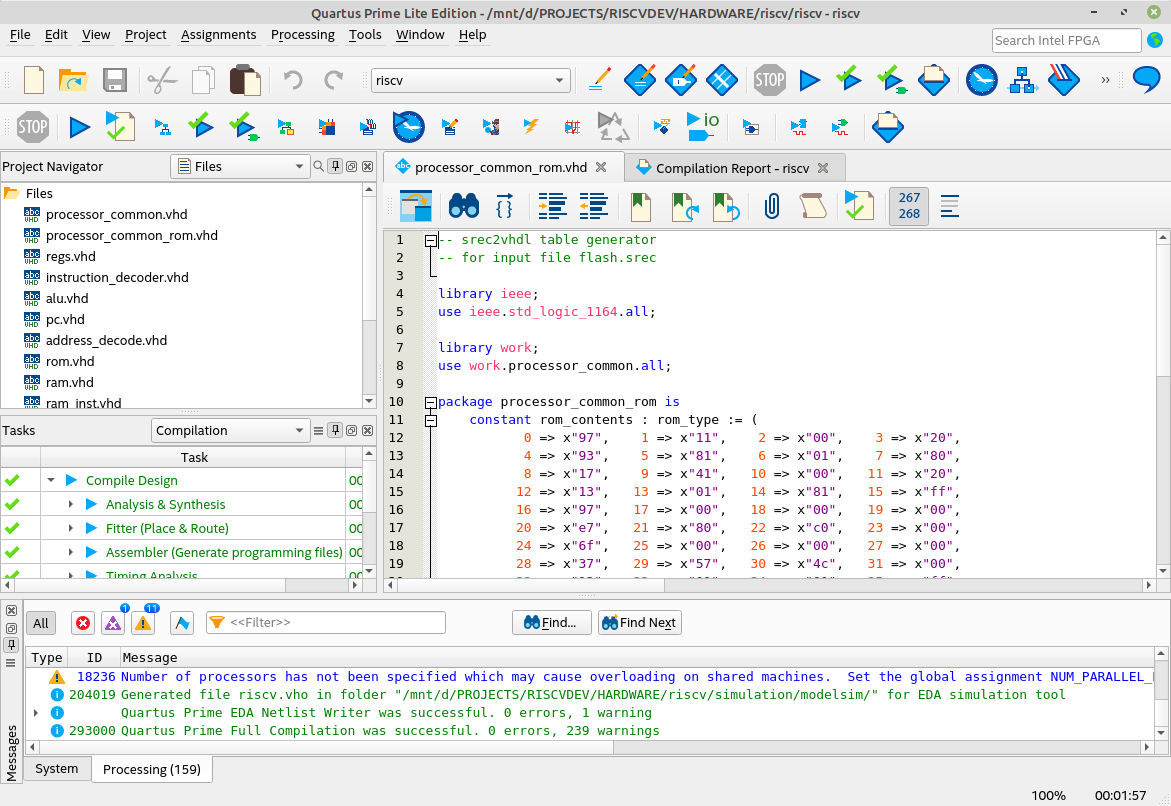
\includegraphics[width=0.85\textwidth]{quartus1}
\caption{Image of the Quartus project (1).}
\label{quartus1}
\end{figure}

\begin{figure}[!ht]
\centering
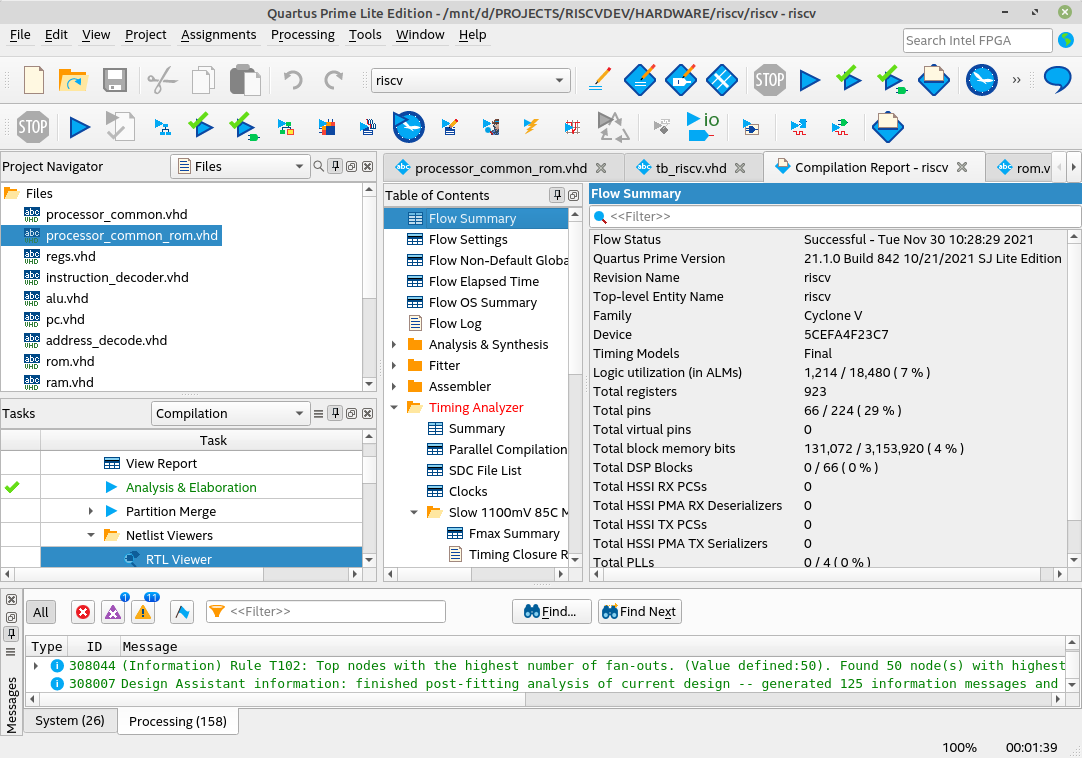
\includegraphics[width=0.85\textwidth]{quartus2}
\caption{Image of the Quartus project (2).}
\label{quartus2}
\end{figure}

\begin{figure}[!ht]
\centering
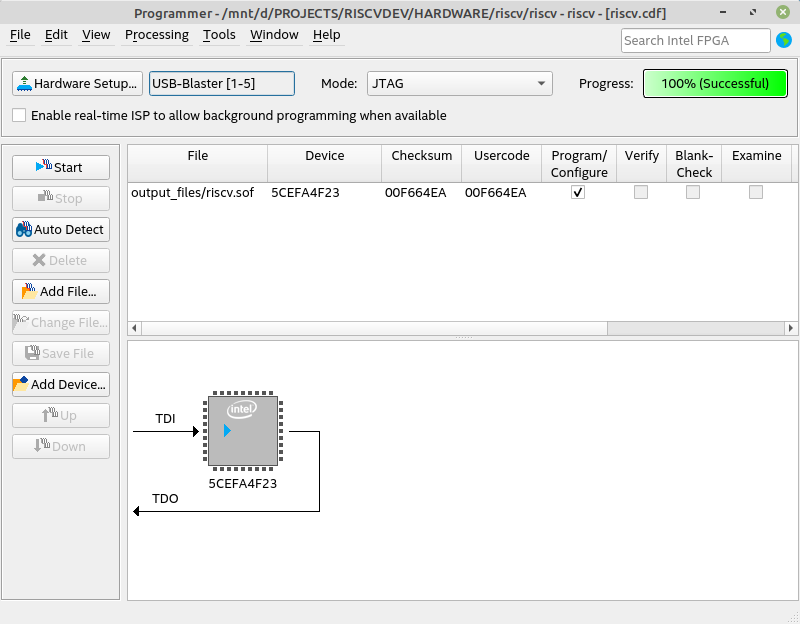
\includegraphics[width=0.85\textwidth]{programmer}
\caption{Image of the programmer.}
\label{programmer}
\end{figure}

\end{itemize}

\section{Implemented system calls}
The \texttt{sbrk/brk} system call, used for allocating RAM memory, is implemented. Note that there is a limited amount of RAM. Note that \texttt{sbrk} is not called by the user. Use \texttt{malloc} et al.

The \texttt{gettimeofday} system call is implemented. It returns the seconds and microseconds since the last reset of the processor. You need to call the \texttt{gettimeofday} C function for proper handling. %Works with the \texttt{clock} C library function.

The \texttt{read} and \texttt{write} system calls are implemented but in turn they call the userland functions \texttt{\_\_io\_getchar} and \texttt{\_\_io\_putchar} functions to read or write a character. Normal use is for the latter two to transmit or receive via the USART. When implemented, \texttt{printf} and \texttt{scanf} can be used.

Other system calls return an error because they cannot fulfill the requested operation, such as \texttt{open}. Note that some system calls are in fact not implemented and return undetermined behavior. 

Note: when using traps, the system calls are handled by a trap handler (by using ECALL). This is the default behavior of the tool chain. When not using traps, the system calls are rerouted to functions in a library. You need to set up your software properly. See the software examples.

\section{Using trap handlers in software}
We provide (see software examples \texttt{interrupt\_direct} and \texttt{interrupt\_vectored}) a basic implementation of trap handlers. The \texttt{universal\_handler} handles all traps (interrupts and exceptions) in direct mode. The entry point (the address loaded in the \texttt{mtvec} CSR) must be set in the \texttt{main} function, as is enabling traps. In vectored mode, interrupts are redirected to their own handlers via a jump table. The start address of the jump table must be set in the \texttt{main} function, and traps must be enabled. The external timer has its own handler called \texttt{external\_timer\_handler}. TIMER1 has its own handler called \texttt{timer1\_cmpt\_handler}. The USART has its own handler called \texttt{usart\_handler}. This handler is used for both receive and transmit interrupts. Note that negating the interrupt request must be done by software in the respective handlers. The interrupt requests is \emph{not} negated by hardware.


\section{VHDL files}
The VHDL description is composed of the following files:

\begin{itemize}
\item \lstinline|processor_common.vhd| -- Common types and constants.
\item \lstinline|processor_common_rom.vhd| -- Description of the ROM contents.
\item \lstinline|address_decode.vhd| -- The address decoder and data router to the memory (ROM, RAM, I/O).
\item \lstinline|alu.vhd| -- Description of the ALU.
\item \lstinline|pc.vhd| -- Description of the Program Counter.
\item \lstinline|instruction_decoder.vhd| -- The instruction decoder.
\item \lstinline|regs.vhd| -- Description of the register file.
\item \lstinline|rom.vhd| -- Description of the ROM interface between the core and the ROM contents.
\item \lstinline|rom_inst.vhd| -- Interface between the ROM contents and the ROM interface. The ROM contents itself is in the file \lstinline|processor_common_rom.vhd|. The ROM contents will be placed in onboard, initialized RAM blocks. 
\item \lstinline|ram.vhd| -- Description of the RAM interface between the address decoder and data router and the onboard RAM.
\item \lstinline|ram_inst.vhd| -- Description of the onboard RAM. Quartus detects this and creates the RAM in onboard, uninitialized RAM blocks.
\item \lstinline|io.vhd| -- Description of the I/O. It contains a 32-bit input register, a 32-bit output register, an USART, a simple timer and the TIME and TIMECMP memory mapped registers.
\item \lstinline|csr.vhd| -- Description of the Control and Status registers.
\item \lstinline|md.vhd| -- Description of the multiply/divide unit.
\item \lstinline|riscv.vhd| -- Top-level description of the processor. Connects all the building blocks to a viable processor.
\item \lstinline|riscv.sdc| -- Constraints file. Sets the target clock frequency.
\item \lstinline|tb_riscv.vhd| -- VHDL testbench to simulate the design.
\item \lstinline|tb_riscv.do| -- QuestaSim/Modelsim command script.
\end{itemize}

There are two architectures for the ALU: a non-optimized, easy-to-follow architecture and an optimized architecture. First impression is that the optimized architecture saves about 500 ALMs in respect to the non-optimized architecture.

There are two architectures for the multiply/divide unit: one with a radix-2 divider and one with a radix-4 divider. The radix-4 divider uses more cells than the radix-2 divider but is faster.

\section{srec2vhdl}
This is a homebrew utility to convert a Motorola S-record file into a VHDL file suitable for inclusion of the processor. The program is called with:

\begin{lstlisting}[language=c]
srec2vhdl [-fbwhqv0] [-i <arg>] inputfile [outputfile]
\end{lstlisting}

\texttt{inputfile} is the S-record file, created by the \texttt{objdump} program. \texttt{outputfile} is the VHDL outputfile. When omitted, \texttt{stdout} is used. There are a number of options:

\begin{itemize}
\item \texttt{-f} makes a full output that directly can be used. If not used, only the ROM table contents itself is produced.
\item \texttt{-w} ROM contents is in words (32 bits).
\item \texttt{-h} ROM contents is in half words (16 bits).
\item \texttt{-b} ROM contents is in bytes (8 bits).
\item \texttt{-v} Verbose output.
\item \texttt{-0} Output unused ROM data as 0 instead of don't care.
\item \texttt{-q} Quiet output, only error messages are displayed.
\item \texttt{-i <arg>} indents each line with \texttt{<arg>} spaces.
\end{itemize}

Note: uninitialized ROM contents is emitted as don't care, except when the \texttt{-0} option is used. Don't cares are set to 0 by Quartus on default.

\section{Software programs}
In de \texttt{CODE} directory, there are a number of software programs available:

\begin{itemize}
\item \texttt{ldfiles} -- contains the linker script. There is one script:
\begin{itemize}
\item \texttt{riscv.ld} -- default linker script: ROM = 64 kB, RAM = 32 kB, I/O = 16 kB.
\end{itemize}
\item \texttt{crt} -- contains the startup files.
\item \texttt{bin} -- contains the binary of \texttt{srec2vhdl}.
\item \texttt{add64} -- simple 64-bit addition. For use in the simulator.
\item \texttt{assembler} -- a simple assembler program. For use in the simulator.
\item \texttt{basel\_problem} -- a program that calculates the sum of the inverses of the squares of natural numbers, up to 1000. For use in the simulator. Used to test the divider.
\item \texttt{clock} -- a simple clock using the CSR TIME and TIMEH registers to fetch the time since last reset. Works on the board.
\item \texttt{double} -- some floating point double computations (seems to work).
\item \texttt{flash} -- flash the DE0-CV board leds (works on the board)
\item \texttt{float} -- some floating point float computations (seems to work).
\item \texttt{global} -- test for globals and local statics with initialization (seems to works).
\item \texttt{hex\_display} -- program that reads 8 switches from the board and display them as a 2-digit hexadecimal value on the 7-segment display. Works on the board.
\item \texttt{interrupt\_direct} -- program to test the interrupt handling using direct mode. Works on the board.
\item \texttt{interrupt\_vectored} -- program to test the interrupt handling using vectored mode. Works on the board.
%\item \texttt{interval} -- program that uses the \texttt{clock} C library function to time 5 seconds since last read. Works only on the pipelined processor. Uses the USART. Works on the board.
\item \texttt{ioadd} -- adds the lower 5 switches to the upper 5 switches and displays the result on the leds. Tests addition, shifting and I/O (works on the board).
\item \texttt{malloc} -- example to test \texttt{malloc} and friends . Works. Used in simulations.
\item \texttt{monitor} -- simple monitor program. Works on the board. Uses strings, USART, RAM, ROM, I/O and \texttt{sprintf} (and therefore \texttt{malloc} et al.).
\item \texttt{mult} -- integer multiplication the hardware md unit. For simulations.
\item \texttt{qsort\_int} -- sorts an integer array using the \texttt{qsort} C library function. Works in simulation.
\item \texttt{riemann\_left} -- calculates the Riemann Left Sum of $\sin^2 x$ from $0$ to $2\pi$. For use in the simulator. The  result must be $\pi$.
\item \texttt{shift} -- shifts. For use in simulations.
\item \texttt{sprintf} -- prints integers, floats/doubles to a string. This is a big binary (seems to work). For simulations.
\item \texttt{string} -- some string functions (seems to work). For simulations.
\item \texttt{syscalls} -- implementing stubs for common system calls (seems to work). Note: \texttt{sbrk} works for \texttt{malloc}, needs more testing.
\item \texttt{testio} -- simple program that copies the input (switches) to the output (leds) (works on the board).
\item \texttt{trig} -- some float trigonometry functions (seems to work). For simulations.
\item \texttt{usart} -- simple USART program. Works on the board.
\item \texttt{usart\_printf} -- simple program that prints an integer, a pointer, a float and a double to the terminal using \texttt{printf}, this is a big binary (works on the board).
\item \texttt{usart\_sprintf} -- simple program that prints an integer, a pointer, a float and a double to the terminal, this is a big binary (works on the board).
\end{itemize} 

Note: we use a lot of the \texttt{volatile} keyword to emit the variables to RAM for easy inspection. You will see compiler warnings from C library functions.

Note that the floating point programs loads (huge) functions from the C library and possibly creates a binary that is too large to fit in the ROM. In that case, the linker will issue an error and does not build the binary. You have to update the data sizes in the VHDL description and update the linker script with suitable data sizes.

When using floats and doubles in \texttt{sprintf}/\texttt{printf}, you need to supply the linker with the \lstinline|-u _printf_float| option. When using floats and doubles in \texttt{sscanf}/\texttt{scanf}, you need to supply the linker with the \lstinline|-u _scanf_float| option. Also, using \texttt{printf} and \texttt{scanf} creates big binaries.

\subsection{Monitor program}
A simple monitor program is available, see the \texttt{monitor} directory in software examples. It makes use of the USART. You need a terminal program like Putty and a USART to USB device for your computer. Currently the following commands are available:

\begin{itemize}
\item \texttt{l} -- set Little Endian (default),
\item \texttt{b} -- set Big endian.
\item \texttt{rw <address>} -- read word at address (4-byte boundary),
\item \texttt{rh <address>} -- read half word at address (2-byte boundary),
\item \texttt{rb <address>} -- read byte at address,
\item \texttt{ww <address> <data>} -- write word at address (4-byte boundary),
\item \texttt{wh <address> <data>} -- write half word at address (2-byte boundary),
\item \texttt{wb <address> <data>} -- write byte at address,
\end{itemize}

\texttt{<address>} and \texttt{<data>} in hexadecimal and Big Endian format. For ROM and RAM read accesses, best set to Little Endian. For I/O accesses, set Big Endian. Make sure to read and write I/O as words. Note that ROM cannot be written.

\section{Address ranges and memory sizes}
By default, the ROM starts at address 0x00000000 and and has a size of 64 kB (16 k words). The Program Counter starts at address 0x00000000. The RAM starts at address 0x20000000 and has a size of 32 kB (8 k words). The stack pointer is set to one address above the last RAM byte, by default at 0x20008000. The I/O starts at address 0xF0000000 and has a size of 16 kB (4 k words).

The ROM, RAM and I/O may be moved to another start location. The Program Counter is started at the correct address. The placement of the ROM is in 256 MB intervals, which are the 4 most significant bits of a 32-bit address. The same holds for the RAM and the I/O. To move the ROM, open the VHDL file \lstinline|processor_common.vhd| and go down to the end of the file. There you will see the following lines:

\begin{lstlisting}[language=VHDL]
-- The highest nibble (4 bits) of the ROM, RAM and I/O
-- This will set the memories at 256 MB intervals
constant rom_high_nibble : std_logic_vector(3 downto 0) := x"0";
constant ram_high_nibble : std_logic_vector(3 downto 0) := x"2";
constant io_high_nibble : std_logic_vector(3 downto 0) := x"F";
\end{lstlisting}

Change the start locations of the memories by changing the constants. Make sure the memories do not overlap. To change the sizes of the memory, look for the lines as shown below:

\begin{lstlisting}[language=VHDL]
-- The ROM
-- NOTE: the ROM is word (32 bits) size.
-- NOTE: data is in Little Endian format (as by the toolchain)
--       for half word and word entities
--       Set rom_size_bits as if it were bytes
-- NOTE: rom_size_bits must be <= 16
constant rom_size_bits : integer := 16;
constant rom_size : integer := 2**(rom_size_bits-2);
type rom_type is array(0 to rom_size-1) of data_type;
-- The contents of the ROM is loaded by processor_common_rom.vhd

-- The RAM
-- NOTE: the RAM is 4x byte (8 bits) size, supporting
--       32-bit Big Endian storage,
--       so we have to recode to support Little Endian.
--       Set ram_size_bits as if it were bytes
-- NOTE: ram_size_bits must be <= 16
constant ram_size_bits : integer := 15;
constant ram_size : integer := 2**(ram_size_bits-2);
-- The type of the RAM block, there are 4 blocks instantiated
type ram_type is array (0 to ram_size-1) of std_logic_vector(7 downto 0);
                    
-- The I/O
-- NOTE: the I/O is word (32 bits) size, Big Endian
--       there is no need to recode the data
--       The I/O can only handle word size access
--       Set io_size_bits as if it were bytes
constant io_size_bits : integer := 8;
constant io_size : integer := 2**(io_size_bits-2);
type io_type is array (0 to io_size-1) of data_type;
\end{lstlisting}

Note that you also have to make changes to the linker script. In the file \texttt{riscv.ld}, at the top you will find the following lines. Change the origins in accordance with the VHDL description.

\begin{lstlisting}
ENTRY( _start )

MEMORY
{
   ROM (rx)   : ORIGIN = 0x00000000, LENGTH = 64K
   RAM (rw)  : ORIGIN = 0x20000000, LENGTH = 32K
   IO (rw)    : ORIGIN = 0xf0000000, LENGTH = 16K
}
\end{lstlisting}

In this setting, the ROM is 64 kB long and the RAM is 32 kB long. Please note that both ROM and RAM bits may not exceed 3,153,920 bits of onboard RAM. For increased ROM and RAM size, typical values may be 128 kB ROM and 64 kB RAM.

Note that we do not use full address decoding for ROM, RAM and I/O. This means that, for example, the ROM is visible multiple times in the address space. This is called \emph{memory foldback}. For the ROM this is at 64 kB intervals. So the contents of address 0x00000000 is also available at address 0x00010000.

\section{Future plans (or not) and issues}
Some future plans:

\begin{itemize}
\item We are \emph{not} planning the C standard.
\item Plans to create a hardcoded bootloader to load programs when the processor is loaded in an FPGA. We need the modify the instruction fetch hardware. Instructions can currently only be fetched from ROM.
\item We strive to implement SPI and I2C, and PWM.
%\item Branches backwards are taken (instruction fetches).
\item We are considering implementing a 5-stage instruction pipeline (this will take time ;-)). This will speed up the clock speed.
\item Implement Supervisor Mode (this will also take some time ;-)).
\item Smaller (in cells) divide unit.
\item Test more functions of the standard and mathematical libraries. Now only a few functions are tested.
\item It is not possible to print \texttt{long long} (i.e. 64-bit) using \texttt{printf} et al. When using the format specifier \texttt{\%lld}, \texttt{printf} just prints \texttt{ld}.
\item The \texttt{mstatus.MIE} bit disables \emph{all} traps, but only interrupts should be disabled.
\item Further optimize the ALU for size and speed.
\item The \texttt{time} (TIMEH:TIME) registers are currently read only.

\end{itemize}

%\section{Author's note}
%I managed to create a basic RISC-V processor within one week, including compiling the GNU C compiler and the created C program examples. Of course, this is not the fastest core available, but it gives a good example on designing a RISC-V processor yourself. Next in line is to make the standard C library work. In the mean time, files will change, so be sure to grab the latest GitHub repository clone.

\appendix
\section{Port I/O}
The processor is equipped with a single 32-bit input and 32-bit output port. There is no data direction register. The reason for this is that the tri-state buffers for bi-direction must be in the top-level entity of the hardware design, making it impossible to use the processor in a greater design. Note that all accesses on the I/O are in Big Endian. This means that bit 31 of the input will be placed in bit 31 of the used variable.

The I/O registers are directly addressable or by a struct. See the listing below.

\begin{lstlisting}[language=C]
#ifndef _IO_H
#define _IO_H

#include <stdint.h>


/* Base address of the I/O */
#define IO_BASE (0xf0000000UL)

/* General purpose I/O */
#define GPIOA_PIN  (*(volatile uint32_t*)(IO_BASE+0x00000000UL))
#define GPIOA_POUT (*(volatile uint32_t*)(IO_BASE+0x00000004UL))

typedef struct {
        volatile uint32_t PIN;
        volatile uint32_t POUT;
} GPIO_struct_t;

#define GPIOA_BASE (IO_BASE+0x00000000UL)

#define GPIOA ((GPIO_struct_t *) GPIOA_BASE)


/* USART (USART1) */
#define USART_DATA (*(volatile uint32_t*)(IO_BASE+0x00000020UL))
#define USART_BAUD (*(volatile uint32_t*)(IO_BASE+0x00000024UL))
#define USART_CTRL (*(volatile uint32_t*)(IO_BASE+0x00000028UL))
#define USART_STAT (*(volatile uint32_t*)(IO_BASE+0x0000002CUL))

typedef struct {
	volatile uint32_t DATA;
	volatile uint32_t BAUD;
	volatile uint32_t CTRL;
	volatile uint32_t STAT;
} USART_struct_t;

#define USART_BASE (IO_BASE+0x00000020UL)

#define USART ((USART_struct_t *) USART_BASE)


/* TIMER (TIMER1) */
typedef struct {
	volatile uint32_t CTRL;
	volatile uint32_t STAT;
	volatile uint32_t CNTR;
	volatile uint32_t CMPT;
} TIMER_struct_t;

#define TIMER1_BASE (IO_BASE+0x00000080UL)
#define TIMER1 ((TIMER_struct_t *) TIMER1_BASE)


/* RISC-V system timer (in I/O) */
#define TIME (*(volatile uint32_t*)(IO_BASE+0x000000f0UL))
#define TIMEH (*(volatile uint32_t*)(IO_BASE+0x000000f4UL))
#define TIMECMP (*(volatile uint32_t*)(IO_BASE+0x000000f8UL))
#define TIMECMPH (*(volatile uint32_t*)(IO_BASE+0x000000fcUL))

typedef struct {
	volatile uint32_t time;
	volatile uint32_t timeh;
} TIME_struct_t;

typedef struct {
	volatile uint32_t timecmp;
	volatile uint32_t timecmph;
} TIMECMP_struct_t;

#endif
\end{lstlisting}

To read the inputs, use:

\begin{lstlisting}[language=C]
uint32_t input;

input = GPIOA->PIN;
\end{lstlisting}

To set the outputs, use:

\begin{lstlisting}[language=C]
uint32_t output = 0xff00ff00;

GPIOA->POUT = output;
\end{lstlisting}

Modifying bits of a I/O register must be done by a read-modify-write cycle. This is \emph{not} atomically handled and can interfere with interrupts! For example, to set bit 2 of POUT, use:

\begin{lstlisting}[language=C]
GPIOA->POUT |= 0x04;
\end{lstlisting}

\section{USART Code}

The USART can send and receive data with one start bit, 7/8/9 data bits, N/E/O parity and 1 or 2 stop bits. Transmission is tested with a baud rate of 9600 bps, 115200 bps and 230400 bps. Send and receive speeds are equal as is the number of data bits, parity and the number of stop bits. There are no auxiliary control signals (e.g. RTS and CTS). There is no embedded FIFO to buffer incoming data. The USART is programmable using I/O registers, see Appendix~\ref{sec:ioregisters}. Note that using a system frequency of 50 MHz, the baud rate cannot be lower than 763 bps.

To initialize the USART, use the code in the listing below:

\begin{lstlisting}[language=C]
/* Frequency of the DE0-CV board */
#define F_CPU (50000000UL)
/* Transmission speed */
#define BAUD_RATE (9600UL)

/* Initialize the Baud Rate Generator */
void usart_init(void)
{
    /* Set baud rate generator */
    USART->BAUD = F_CPU/BAUD_RATE-1;
}
\end{lstlisting}

To send a single character with waiting, use the code in the listing below:

\begin{lstlisting}[language=C]
/* Send one character over the USART */
void usart_putc(int ch)
{
    /* Transmit data */
    USART->DATA = (uint8_t) ch;
            
    /* Wait for transmission end */
    while ((USART->STAT & 0x10) == 0);
}
\end{lstlisting}

To send a null-terminated string, use the code in the listing below:

\begin{lstlisting}[language=C]
/* Send a null-terminated string over the USART */
void usart_puts(char *s)
{
    if (s == NULL)
    {
        return;
    }

    while (*s != '\0')
    {
        usart_putc(*s++);
    }
}
\end{lstlisting}

To wait for a character reception, use the code in the listing below:

\begin{lstlisting}[language=C]
/* Get one character from the USART in
 * blocking mode */
int usart_getc(void)
{
        /* Wait for received character */
        while ((USART->STAT & 0x04) == 0);

        /* Return 8-bit data */
        return USART->DATA & 0x000000ff;
}
\end{lstlisting}

To receive a string from the USART, including some simple line editing, use the code in the listing below:

\begin{lstlisting}[language=C]
/* Gets a string terminated by a newline character from usart
 * The newline character is not part of the returned string.
 * The string is null-terminated.
 * A maximum of size-1 characters are read.
 * Some simple line handling is implemented */
int usart_gets(char buffer[], int size) {
    int index = 0;
    char chr;

    while (1) {
        chr = usart_getc();
        switch (chr) {
            case '\n':
            case '\r':  buffer[index] = '\0';
                        usart_puts("\r\n");
                        return index;
                        break;
            /* Backspace key */
            case 0x7f:
            case '\b':  if (index>0) {
                            usart_putc(0x7f);
                            index--;
                        } else {
                            usart_putc('\a');
                        }
                    break;
            /* control-U */
            case 21:    while (index>0) {
                            usart_putc(0x7f);
                            index--;
                        }
                        break;
            /* control-C */
            case 0x03:  usart_puts("<break>\r\n");
                        index=0;
                        break;
            default:    if (index<size-1) {
                            if (chr>0x1f && chr<0x7f) {
                                buffer[index] = chr;
                                index++;
                                usart_putc(chr);
                            }
                        } else {
                            usart_putc('\a');
                        }
                        break;
        }
    }
    return index;
}
\end{lstlisting}

When printing a C newline, you have to use:

\begin{lstlisting}[language=C]
usart_puts("\r\n");
\end{lstlisting}

This will set the cursor to the beginning of a new line. Here, \lstinline|\r| returns the cursor to the beginning of the current line and \lstinline|\n| advances the cursor to the next line. Some terminal emulation programs can be instructed to move to the beginning of a new line with only \lstinline|\n|.

For working with the USART on board of the processor, you need an USB-to-USART device with TTL (3.3 V) converter. An example is shown in Figure~\ref{fig:usb-usart-ttl}.

\begin{figure}[!ht]
\centering
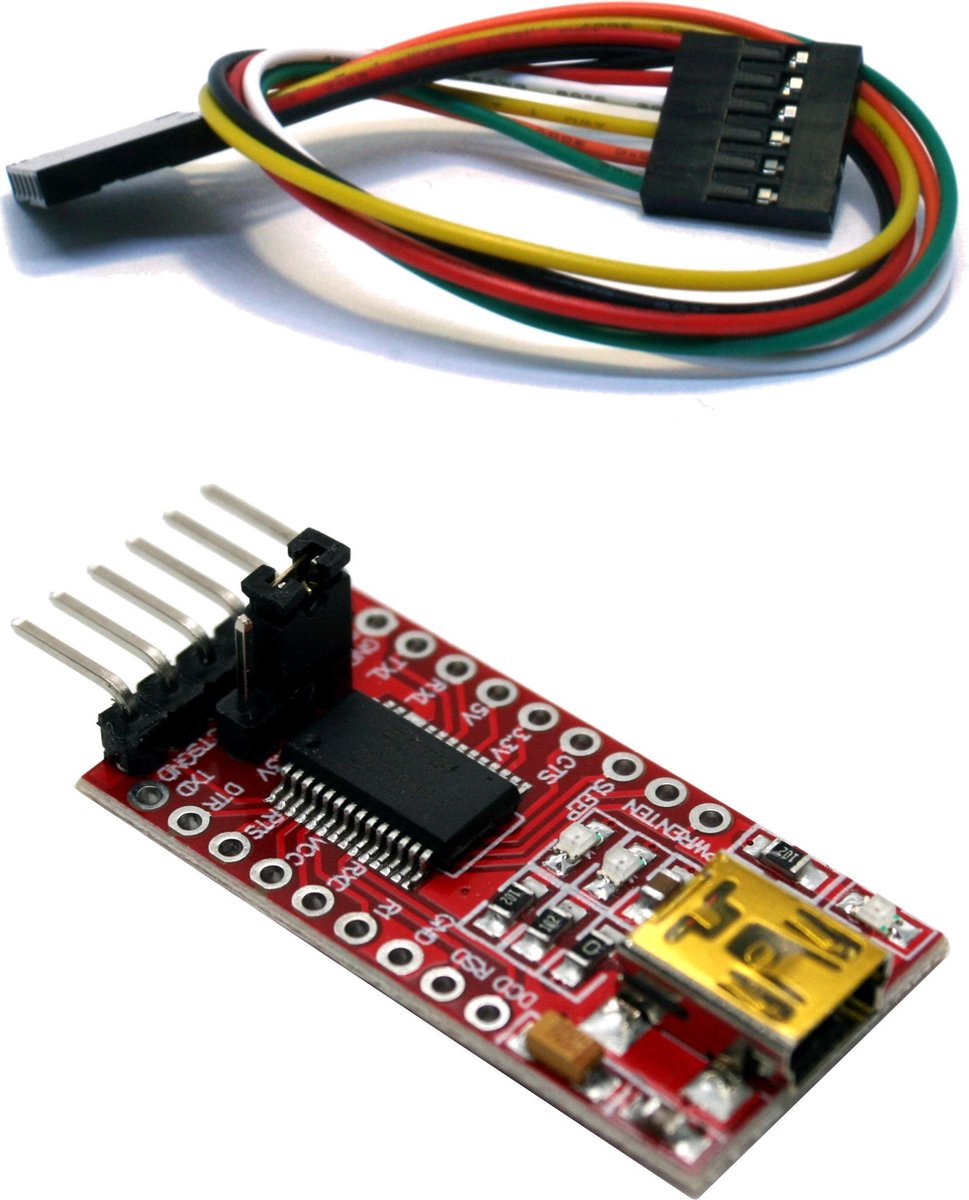
\includegraphics[scale=0.1]{usb-usart-ttl}
\caption{An USB-to-USART converter. Make sure that the voltages do not exceed 3.3 V.}
\label{fig:usb-usart-ttl}
\end{figure}


\section{TIMER1 code}
Based on a frequency of 50$\,$MHz, the following code will set TIMER1 interrupt on 0,5 s intervals:

\begin{lstlisting}[language=C]
/* Activate TIMER1 with a cycle of 2 Hz */
/* for a 50 MHz clock. Use interrupt. */
TIMER1->CMPT = 24999999;
/* Bit 0 = enable, bit 4 is interrupt enable */
TIMER1->CTRL = (1<<4)|(1<<0);
\end{lstlisting}

\section{The external \texttt{time} registers}
The \texttt{time} registers (TIME, TIMEH, TIMEMCP and TIMECMPH) can be accessed via the I/O and are therefore memory mapped. The following code reads in the current time and increments the compare registers with a certain \emph{delta}. Whenever TIMEH:TIME is greater than or equal to TIMEH:TIME, an interrupt request is asserted. Negating the interrupt request is accomplished by writing a value greater than the time registers to the compare registers.

\begin{lstlisting}[language=C]
register uint32_t time;
register uint32_t timeh;

/* Fetch current time */
do {
        timeh = TIMEH;
        time  = TIME;
} while (timeh != TIMEH);

/* Fetch current time */
register uint64_t cur_time;
cur_time = ((uint64_t)timeh << 32) | (uint64_t)time;

/* Add delta */
cur_time += external_timer_delta;

/* Set TIMECMP to maximum */
TIMECMPH = -1;
TIMECMP = -1;

/* Store new TIMECMP */
TIMECMP = (uint32_t)(cur_time & 0xffffffff);
TIMECMPH = (uint32_t)(cur_time>>32);
\end{lstlisting}

Normally, this code is placed in the interrupt handler. These registers are read-only shadowed to the CSR time registers.

\section{I/O registers}
\label{sec:ioregisters}
This is a list of currently supported I/O addresses. 
The default start address is 0xF0000000. The offset is given in bytes. Note that the I/O can only be accesses on 4-byte boundaries and on word size accesses.

\subsection{General purpose I/O}

\begin{register}{H}{Port A input register PIN}{0x00}%
\label{pinx}%
\regfield{PIN}{32}{0}{{0}}% READ_ONLY
\reglabel{Reset}\regnewline%
\end{register}
\begin{regdesc}[0.6\textwidth]\begin{reglist}[000000000]
\itemsep-1.5ex
\item[Note:] This I/O register can only be read.
\end{reglist}\end{regdesc}

\begin{register}{H}{Port A output register POUT}{0x04}%
\label{poutx}%
\regfield{POUT}{32}{0}{{0}}
\reglabel{Reset}\regnewline%
\end{register}
\begin{regdesc}[0.6\textwidth]\begin{reglist}[000000000]
\itemsep-1.5ex
\item[Write] The data is written to the output pins.
\item[Read] The last entered data is read back.
\end{reglist}\end{regdesc}

\subsection{USART}

\begin{register}{H}{USART data register USART\_DATA}{0x20}
\label{usartdata}
\regfield{Reserved}{22}{9}{{0}}%
\regfield{Data}{9}{0}{{0}}%
\reglabel{Reset}\regnewline%
\end{register}
\begin{regdesc}[0.6\textwidth]\begin{reglist}[000000000]
\itemsep-1.5ex
\item[Write] The data is written to an internal buffer and transmitted.
\item[Read] The last received data is read.
\end{reglist}\end{regdesc}
\hspace*{2cm}Size depends on the Size field in the USART Control Register.

\begin{register}{H}{USART baud rate register USART\_BAUD}{0x24}
\label{usartbaud}
\regfield{Rerserved}{16}{16}{{0}}%
\regfield{Prescaler}{16}{0}{{0}}%
\reglabel{Reset}\regnewline%
\end{register}
\begin{regdesc}[0.6\textwidth]\begin{reglist}[000000000]
\itemsep-1.5ex
\item[Prescaler] Baud rate = $\dfrac{f_{system}}{\textrm{prescaler}+1}$
\end{reglist}\end{regdesc}

\begin{register}{H}{USART control register USART\_CTRL}{0x28}
\label{usartctrl}
\regfield{Reserved}{24}{8}{{0}}%
\regfield{TCIE}{1}{7}{{1}}%
\regfield{RCIE}{1}{6}{{1}}%
\regfield{Parity}{2}{4}{{0}}%
\regfield{Size}{2}{2}{{0}}%
\regfield{Reserved}{1}{1}{{0}}%
\regfield{SP}{1}{0}{{0}}
\reglabel{Reset}\regnewline%
\end{register}
\begin{regdesc}[0.6\textwidth]\begin{reglist}[00000]
\itemsep-1.5ex
\item[TCIE] Transmit character interrupt enable.
\item[RCIE] Receive character interrupt enable.
\item[Parity] 00: none, 10: even, 11: odd.
\item[Size] 00: 8 bits, 10: 9 bits, 11: 7 bits, excluding the parity.
\item[SP] 0: one stop bit, 1: two stop bits.
%\item[Stop Bits] Meaning
%\item[0] 1 Stop bit
%\item[1] 2 Stop bits
%\item
%\item[Parity] Meaning
%\item[00] No parity
%\item[01] Reserved
%\item[10] Even parity
%\item[11] Odd parity
%\item
%\item[Data bits]
%\item[0] 8 bits
%\item[9] 9 bits
\end{reglist}\end{regdesc}

\begin{register}{H}{USART status register USART\_STAT}{0x2c}
\label{usartstat}
\regfield{Reserved}{27}{5}{{0}}%
\regfield{TC}{1}{4}{{0}}%
\regfield{PE}{1}{3}{{0}}%
\regfield{RC}{1}{2}{{0}}%
\regfield{RF}{1}{1}{{0}}%
\regfield{FE}{1}{0}{{0}}%
\reglabel{Reset}\regnewline%
\end{register}
\begin{regdesc}[0.8\textwidth]\begin{reglist}[0000]
\itemsep-1.5ex
\item[TC] Transmit completed. Set directly to 1 when a character was transmitted. Automatically cleared when writing new character to the data register or when writing 0 in the TC bit in \mbox{USART\_STAT}.
\item[PE] Parity error. Set to 1 if parity is enabled and there is a parity error while receiving. Automatically cleared when data register is read or when writing 0 in the PE bit in USART\_STAT.
\item[RC] Receive completed. Set to 1 when a character was received. Automatically cleared when data register is read or when writing 0 in the RC bit in USART\_STAT.
\item[RF] Receive failed. Set to 1 when failed receiving (invalid start bit). Automatically cleared when data register is read or when writing 0 in the RF bit in USART\_STAT.
\item [FE] Frame error. Set to 1 when a low is detected at the position of the (first) stop bit. Automatically cleared when data register is read or writing a 0 in the FE bit in USART\_STAT.
\end{reglist}\end{regdesc}

\subsection{TIMER1}
\begin{register}{H}{TIMER1 control register TIMER1\_CTRL}{0x80}
\label{timer1ctrl}
\regfield{Reserved}{27}{5}{{0}}%
\regfield{TIE}{1}{4}{{0}}%
\regfield{Reserved}{3}{1}{{000}}%
\regfield{EN}{1}{0}{{0}}%
\reglabel{Reset}\regnewline%
\end{register}
\begin{regdesc}[0.8\textwidth]\begin{reglist}[0000]
\itemsep-1.5ex
\item[EN] Enable the timer
\item[TIE] Timer compare match interrupt enable
\end{reglist}\end{regdesc}

\begin{register}{H}{TIMER1 status register TIMER1\_STAT}{0x84}
\label{timer1stat}
\regfield{Reserved}{27}{5}{{0}}%
\regfield{TCI}{1}{4}{{0}}%
\regfield{Reserved}{4}{0}{{0000}}%
\reglabel{Reset}\regnewline%
\end{register}
\begin{regdesc}[0.8\textwidth]\begin{reglist}[0000]
\itemsep-1.5ex
\item[TCI] Timer compare match interrupt. Set to 1 on compare match between the timer Count register and the Compare Match register. Must be cleared by software by writing a 0.
\end{reglist}\end{regdesc}

\begin{register}{H}{TIMER1 count register TIMER1\_CNTR}{0x88}
\label{timer1cntr}
\regfield{CNTR}{32}{0}{{0}}%
\reglabel{Reset}\regnewline%
\end{register}
\begin{regdesc}[0.8\textwidth]\begin{reglist}[0000]
\itemsep-1.5ex
\item[CNTR] This register holds the counted clock pulses on the timer. This register may be written by software. Rolls over every $2^{32}/f_{clk}$ seconds.
\end{reglist}\end{regdesc}

\begin{register}{H}{TIMER1 compare timer register TIMER1\_CMPT}{0x8c}
\label{timer1cmpt}
\regfield{CMPT}{32}{0}{{0}}%
\reglabel{Reset}\regnewline%
\end{register}
\begin{regdesc}[0.8\textwidth]\begin{reglist}[0000]
\itemsep-1.5ex
\item[CMPT] This register holds the value at which the counter register is compared. On CNTR compares to greater than or equal to CMPT, the counter register will be cleared and the TCI flag will be set (both in the next clock cycle).
\end{reglist}\end{regdesc}

\begin{register}{H}{TIME external timer register TIME}{0xf0}
\label{time}
\regfield{TIME}{32}{0}{{0}}%
\reglabel{Reset}\regnewline%
\end{register}
\begin{regdesc}[0.8\textwidth]\begin{reglist}[0000]
\itemsep-1.5ex
\item This register holds the low 32 bits of the external timer. Currently read-only.
\end{reglist}\end{regdesc}

\begin{register}{H}{TIMEH external timer register TIME}{0xf4}
\label{timeh}
\regfield{TIMEH}{32}{0}{{0}}%
\reglabel{Reset}\regnewline%
\end{register}
\begin{regdesc}[0.8\textwidth]\begin{reglist}[0000]
\itemsep-1.5ex
\item This register holds the upper 32 bits of the external timer. Currently read-only.
\end{reglist}\end{regdesc}

\begin{register}{H}{TIMECMP external timer compare register TIMECMP}{0xf8}
\label{timecmp}
\regfield{TIMECMP}{32}{0}{{0}}%
\reglabel{Reset}\regnewline%
\end{register}
\begin{regdesc}[0.8\textwidth]\begin{reglist}[0000]
\itemsep-1.5ex
\item This register holds the low 32 bits of the external timer compare register.
\end{reglist}\end{regdesc}

\begin{register}{H}{TIMECMPH external timer compare register TIMECMP}{0xfc}
\label{timecmph}
\regfield{TIMECMPH}{32}{0}{{0}}%
\reglabel{Reset}\regnewline%
\end{register}
\begin{regdesc}[0.8\textwidth]\begin{reglist}[0000]
\itemsep-1.5ex
\item This register holds the upper 32 bits of the external timer compare register.
\end{reglist}\end{regdesc}

%\lstinputlisting[language=VHDL,basicstyle=\small\ttfamily]{../HARDWARE/riscv-pipe-csr-md-lic/alu.vhd}
%\lstinputlisting[language=VHDL,basicstyle=\small\ttfamily]{../HARDWARE/riscv-pipe-csr-md-lic/processor_common.vhd}

%\lstinputlisting[language=VHDL,basicstyle=\small\ttfamily]{../HARDWARE/riscv-pipe-csr-md-lic/processor_common_rom.vhd}


\end{document}